\subsection{Regresja liniowa}
Na początku przeprowadzamy prostą regresję liniową:

\begin{figure}[H]
    \centering
    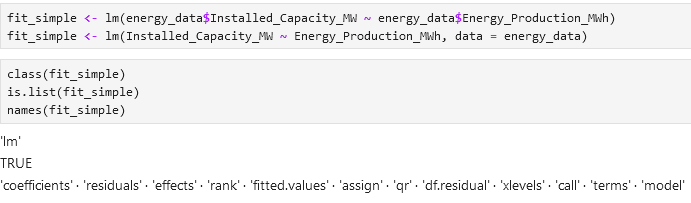
\includegraphics[width=0.9\linewidth]{lab1/obraz.png}
    \caption{Zmienna objaśniana - Installed Capacity MW. Zmienna objaśniająca - Energy Production MWh}
    \label{fig:regression}
\end{figure}

\begin{figure}[H]
    \centering
    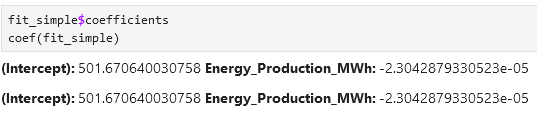
\includegraphics[width=0.9\linewidth]{lab1/obraz2.png}
    \caption{Współczynniki regresji}
    \label{fig:coefficients}
\end{figure}

\begin{figure}[H]
    \centering
    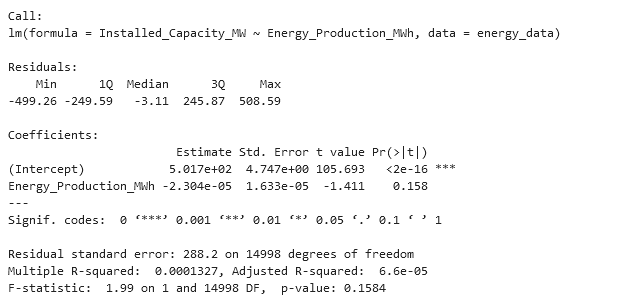
\includegraphics[width=0.9\linewidth]{lab1/obraz3.png}
    \caption{Podsumowanie regresji liniowej}
    \label{fig:summary}
\end{figure}

\begin{figure}[H]
    \centering
    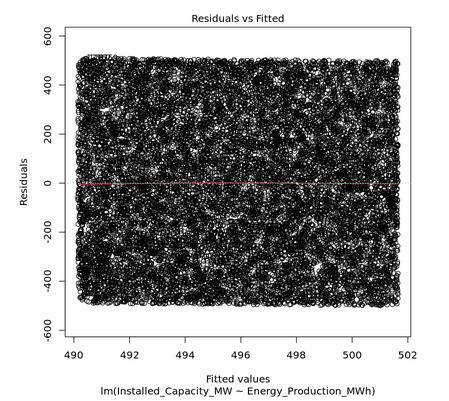
\includegraphics[width=0.9\linewidth]{lab1/obraz4.png}
    \caption{Wartości rzeczywiste vs przewidywane}
    \label{fig:real_vs_predicted}
\end{figure}

\begin{figure}[H]
    \centering
    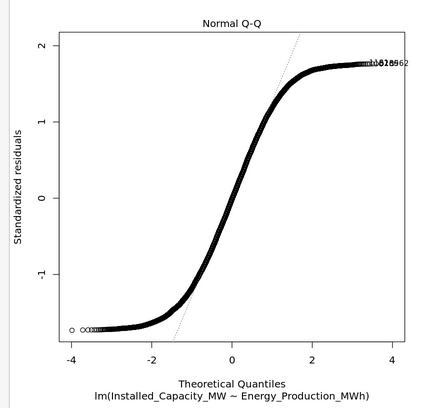
\includegraphics[width=0.9\linewidth]{lab1/obraz5.png}
    \caption{Reszty regresji}
    \label{fig:residuals}
\end{figure}

\begin{figure}[H]
    \centering
    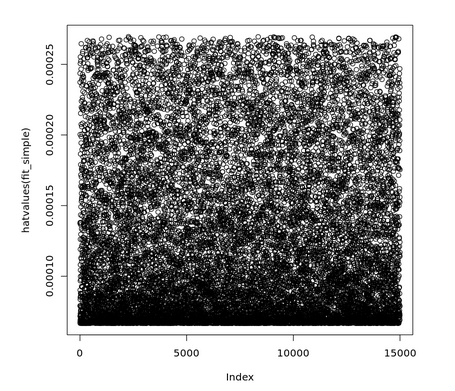
\includegraphics[width=0.9\linewidth]{lab1/obraz6.png}
    \caption{Heat values}
    \label{fig:heat_values}
\end{figure}

\subsection{Regresja wielokrotna}
Przejdźmy do regresji wielokrotnej. Będziemy przewidywać wartość \textbf{Installed\_Capacity\_MW} na podstawie zmiennych \textbf{Energy\_Production\_MWh} i \textbf{Energy\_Consumption\_MWh}.

\begin{Rcode}
fit_la <- lm(energy_data$Installed_Capacity_MW ~ energy_data$Energy_Production_MWh + energy_data$Energy_Consumption_MWh)
\end{Rcode}

\begin{figure}[H]
    \centering
    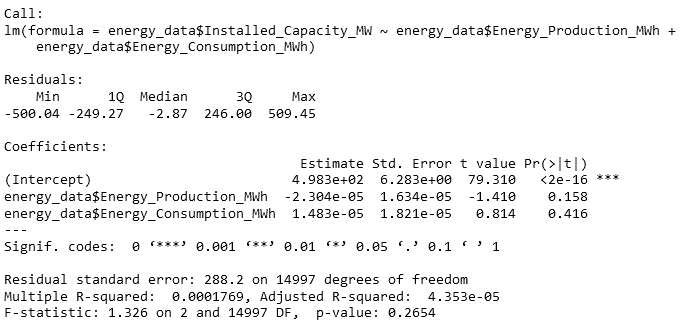
\includegraphics[width=1\linewidth]{lab1/obraz9.png}
    \caption{Enter Caption}
    \label{fig:enter-label}
\end{figure}

Przeprowadźmy teraz regresję wielokrotną dla jednej zmiennej dla pozostałych zmiennych liczbowych:

\begin{Rcode}
numerical_data <- energy_data[, sapply(energy_data, is.numeric)]
fit_all <- lm(Installed_Capacity_MW ~ ., data = numerical_data)
\end{Rcode}

\begin{figure}[H]
    \centering
    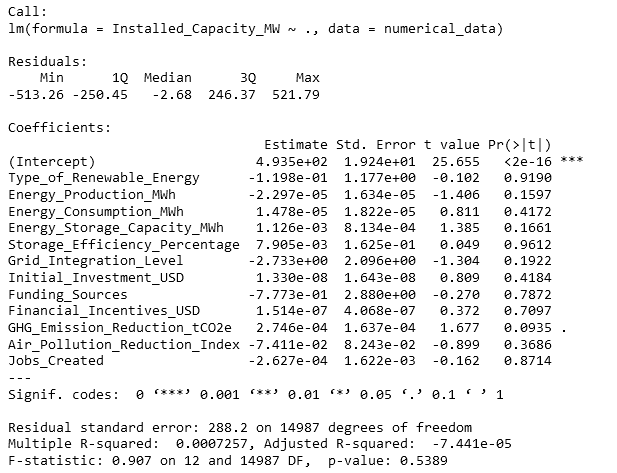
\includegraphics[width=1\linewidth]{lab1/obraz10.png}
    \caption{Enter Caption}
    \label{fig:enter-label}
\end{figure}

\begin{figure}[H]
    \centering
    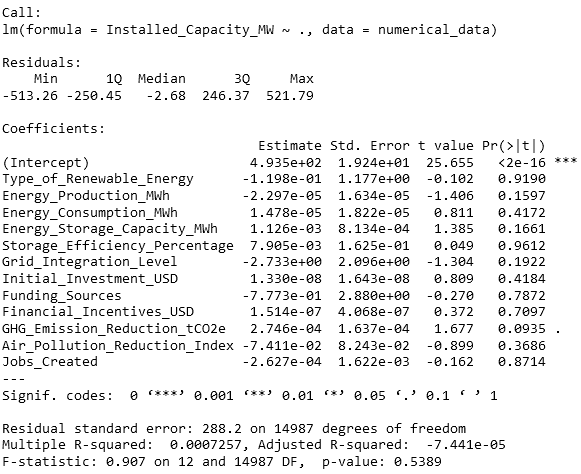
\includegraphics[width=1\linewidth]{lab1/obraz11.png}
    \caption{Enter Caption}
    \label{fig:enter-label}
\end{figure}

A teraz bez zmiennej Grid\_Integration\_Level:

\begin{Rcode}
fit_no_grid_int <- update(fit_all, ~ . - Grid_Integration_Level)
summary(fit_no_grid_int)
\end{Rcode}

\begin{figure}[H]
    \centering
    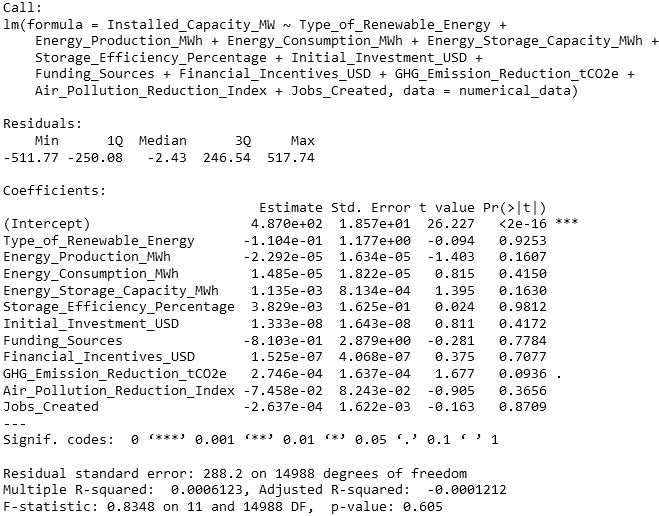
\includegraphics[width=1\linewidth]{lab1/obraz12.png}
    \caption{Enter Caption}
    \label{fig:enter-label}
\end{figure}

Wybrane przedziały ufności:

\begin{figure}[H]
    \centering
    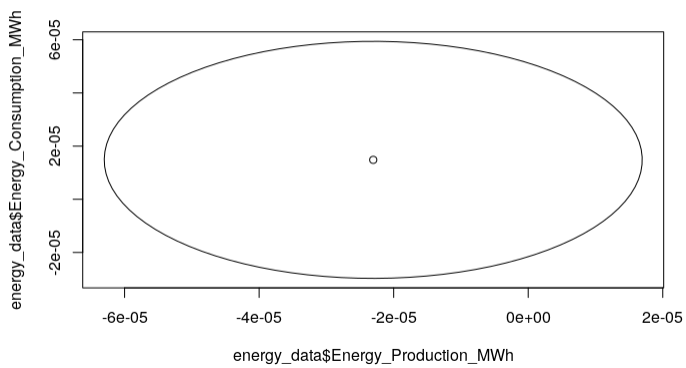
\includegraphics[width=1\linewidth]{lab1/obraz13.png}
    \caption{Enter Caption}
    \label{fig:enter-label}
\end{figure}

Sprawdźmy jeszcze jak poradzi sobie regresja wielomianowa (5 stopnia):

\begin{Rcode}
anova(fit_simple, fit_l2)
fit_l5 <- lm(energy_data$Energy_Consumption_MWh ~ poly(energy_data$Energy_Production_MWh, 5))
summary(fit_l5)
summary(lm(Energy_Production_MWh ~ log(Energy_Consumption_MWh), data = energy_data))
\end{Rcode}

\begin{figure}[H]
    \centering
    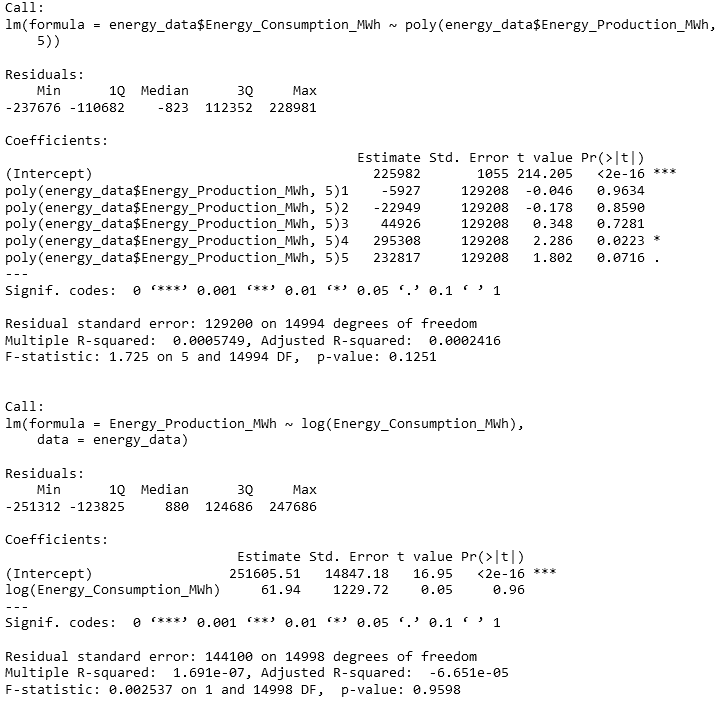
\includegraphics[width=1\linewidth]{lab1/obraz14.png}
    \caption{Enter Caption}
    \label{fig:enter-label}
\end{figure}